\documentclass[../main.tex]{subfiles}
 
\begin{document}

\newpage

\section{Usage}

\subsection{Building}

Before enabling the Subfiling VFD, it has a few requirements that have to be
satisfied:

\begin{itemize}
\item The VFD requires that HDF5 is built with parallel support using an MPI
implementation that supports at least the MPI-3 standard,

\item The VFD requires a C11-compliant compiler since it currently makes use
of the C11 atomic type primitives from \texttt{stdatomic.h},

\item The VFD is officially only supported on Linux systems due to
the direct use of pthreads for threading. While the VFD may work under
MinGW or similar, this is not tested.
\end{itemize}

If these requirements are satisfied, the Subfiling VFD can be enabled by building using either CMake, Section \ref{subsubsec:cmake}, or Autotools, Section  \ref{subsubsec:autotools}. HDF5
will check for these requirements and then build the VFD into the library.

\subsubsection{\label{subsubsec:cmake}CMake}

\begin{minted}{bash}
cmake -DHDF5_ENABLE_PARALLEL=ON -DHDF5_ENABLE_SUBFILING_VFD=ON ..
\end{minted}

\subsubsection{\label{subsubsec:autotools}Autotools}

\begin{minted}{bash}
./configure --enable-parallel --enable-subfiling-vfd=yes
\end{minted}

\subsection{Loading}

To load and use the Subfiling VFD within an HDF5 application, a few steps must
first be taken to ensure proper operation.

\subsubsection{Initialize MPI with MPI\_THREAD\_MULTIPLE threading support}
\label{sec:req1}

The Subfiling VFD uses a combination of MPI and threading internally to achieve
its purpose. This means that a parallel HDF5 application wishing to use the
Subfiling VFD should call \texttt{MPI\_Init\_thread} (rather than \texttt{MPI\_Init})
at the beginning of the application. Further, any particular thread created by the
VFD may make MPI calls at any time, so the VFD requires that MPI is initialized
with support for this behavior by passing the \texttt{MPI\_THREAD\_MULTIPLE}
flag to \texttt{MPI\_Init\_thread}. See \ref{ex:ex1} for a minimal example of
using the Subfiling VFD which does this. After calling \texttt{MPI\_Init\_thread},
the application should always check that the level of threading support provided
by the MPI implementation is at least \texttt{MPI\_THREAD\_MULTIPLE} before
attempting to use the VFD. For example:

\begin{minted}{hdf5-c-lexer.py:HDF5CLexer -x}
int
main(int argc, char **argv)
{
    int mpi_thread_required = MPI_THREAD_MULTIPLE;
    int mpi_thread_provided = 0;

    if (MPI_SUCCESS != MPI_Init_thread(&argc, &argv,
                                       mpi_thread_required,
                                       &mpi_thread_provided))
        return -1;

    if (mpi_thread_provided < mpi_thread_required)
        return -1;

    ...

    MPI_Finalize();

    return 0;
}
\end{minted}

Failing to perform this check may result in odd and difficult to diagnose errors
when the MPI implementation doesn't provide the \texttt{MPI\_THREAD\_MULTIPLE}
level of threading support.

\textbf{NOTE:} If using MPICH for an MPI implementation, it may be necessary on
some systems to set the \texttt{MPICH\_MAX\_THREAD\_SAFETY} environment variable
to "multiple", as in:

\begin{minted}{bash}
export MPICH_MAX_THREAD_SAFETY=multiple
\end{minted}

in order to have access to the required \texttt{MPI\_THREAD\_MULTIPLE} level of
threading support when calling \texttt{MPI\_Init\_thread}.

\subsubsection{Set any MPI parameters}
\label{sec:req2}

The Subfiling VFD checks for any specially set MPI parameters during initialization,
so if the HDF5 application needs to use a special MPI Communicator and/or MPI Info
object, it should make use of the \texttt{H5Pset\_mpi\_params} API routine to set
those MPI parameters on a \Gls{FAPL} to be used for file access before making calls
to any Subfiling VFD-related API routines. In the absence of any specially set MPI
parameters, the Subfiling VFD will default to using \texttt{MPI\_COMM\_WORLD} for the
MPI Communicator and \texttt{MPI\_INFO\_NULL} for the MPI Info object.

\begin{minted}{hdf5-c-lexer.py:HDF5CLexer -x}
hid_t fapl_id = H5Pcreate(H5P_FILE_ACCESS);
/* Set any special MPI parameters */
H5Pset_mpi_params(fapl_id, MPI_COMM_WORLD, MPI_INFO_NULL);
\end{minted}

\subsubsection{Set Subfiling VFD on a FAPL}

Once these initial steps have been performed within an HDF5 application, using
the Subfiling VFD simply entails setting up a \Gls{FAPL} with Subfiling VFD access,
as in:

\begin{minted}{hdf5-c-lexer.py:HDF5CLexer -x}
hid_t fapl_id = H5Pcreate(H5P_FILE_ACCESS);
/* Set any special MPI parameters */
H5Pset_mpi_params(fapl_id, MPI_COMM_WORLD, MPI_INFO_NULL);
/* Optional Subfiling configuration can be provided rather than NULL */
H5Pset_fapl_subfiling(fapl_id, NULL);
hid_t file_id = H5Fcreate("file.h5", H5F_ACC_TRUNC, H5P_DEFAULT, fapl_id);
\end{minted}

See sections \ref{ex:ex1} and \ref{ex:ex2} for minimal examples of using the Subfiling VFD with
default and custom configurations.

\subsubsection{Load by environment variable}

Though mostly for testing purposes, the Subfiling VFD can also be loaded by setting
the \texttt{HDF5\_DRIVER} environment variable, as in:

\begin{minted}{bash}
export HDF5_DRIVER=subfiling
\end{minted}

When the Subfiling VFD is loaded this way, the only way to configure the VFD in a non-default
manner is through the use of environment variables, as described in section \ref{sec:envvars}.

\textbf{NOTE:} The HDF5 application must still fulfill the requirements in the previous
sections (\ref{sec:req1} and \ref{sec:req2}) to load the Subfiling VFD in this manner.

\subsection{Configuring}

There are two main ways to configure the Subfiling VFD: providing a Subfiling configuration
structure to the \texttt{H5Pset\_fapl\_subfiling} API routine or setting environment variables.

\subsubsection{By File Access Property List}

The \texttt{H5Pset\_fapl\_subfiling} API routine accepts a pointer to a \texttt{H5FD\_subfiling\_config\_t}
structure for configuration (defined in \ref{ref:h5fd_subfiling_config_t}). If this parameter
is \texttt{NULL}, the Subfiling VFD will use the default settings of:

\begin{itemize}
\item Default "IOC" VFD used for the I/O Concentrator VFD
\item 32MiB data stripe size
\item 1 I/O Concentrator per machine node
\item 4 worker threads per I/O Concentrator
\end{itemize}

\subsubsection{By environment variables}
\label{sec:envvars}

The Subfiling VFD can also be configured with a few different environment variables that
generally take precedence over any Subfiling configuration parameters set on a FAPL:

\begin{itemize}
\item \texttt{H5FD\_SUBFILING\_STRIPE\_SIZE} - This environment variable controls the size of
the data stripes written to subfiles. It is interpreted as a \texttt{long long} value and must
be $> 0$.

\item \texttt{H5FD\_SUBFILING\_IOC\_PER\_NODE} - This environment variable controls the number
of I/O Concentrators that will be assigned to each machine node. It is interpreted as a \texttt{long}
value and must be $> 0$.

\item \texttt{H5FD\_SUBFILING\_IOC\_SELECTION\_CRITERIA} - This environment variable is intended
to be used in conjunction with the I/O Concentrator selection method specified in a Subfiling
configuration structure set on a \Gls{FAPL}. It enables the user to specify extra criteria for
how the Subfiling VFD should operate when selection I/O Concentrators. Refer to
\href{https://github.com/HDFGroup/hdf5/blob/develop/src/H5FDsubfiling/H5FDsubfiling.h}{the Subfiling VFD header}
for more information on allowed values for this environment variable.

\item \texttt{H5FD\_SUBFILING\_SUBFILE\_PREFIX} - This environment variable allows setting of a
prefix that is prepended to the filenames generated for subfiles. It is interpreted as a string
value.

\item \texttt{H5FD\_IOC\_THREAD\_POOL\_SIZE} - This environment variable controls the number of
worker threads per I/O Concentrator. It is interpreted as an \texttt{int} value and must be $> 0$.
\end{itemize}

\subsection{Minimal example}

The following is a minimal example of creating a Subfiling-based HDF5 file
with the default Subfiling configuration of a 32MiB stripe size, 1 I/O Concentrator
per machine node and 4 worker threads per I/O Concentrator. 

\label{ex:ex1}
\begin{minted}{hdf5-c-lexer.py:HDF5CLexer -x}
#include "hdf5.h"

int
main(int argc, char **argv)
{
    MPI_Comm comm = MPI_COMM_WORLD;
    MPI_Info info = MPI_INFO_NULL;
    hid_t    file_id = H5I_INVALID_HID;
    hid_t    fapl_id = H5I_INVALID_HID;
    int      mpi_thread_required = MPI_THREAD_MULTIPLE;
    int      mpi_thread_provided = 0;

    /* Initialize MPI with threading support */
    MPI_Init_thread(&argc, &argv, mpi_thread_required, &mpi_thread_provided);
    if (mpi_thread_provided != mpi_thread_required)
        MPI_Abort(comm, -1);

    /*
     * Set up File Access Property List with MPI
     * parameters for the Subfiling VFD to use
     */
    fapl_id = H5Pcreate(H5P_FILE_ACCESS);
    H5Pset_mpi_params(fapl_id, comm, info);

    /*
     * Set Subfiling VFD on FAPL using default settings
     * (use IOC VFD, 1 IOC per node, 32MiB stripe size)
     */
    H5Pset_fapl_subfiling(fapl_id, NULL);
    
    /*
     * Create a new Subfiling-based HDF5 file
     */
    file_id = H5Fcreate("my_h5_file.h5", H5F_ACC_TRUNC, H5P_DEFAULT, fapl_id);

    /* Close/free resources */
    H5Pclose(fapl_id);
    H5Fclose(file_id);

    MPI_Finalize();

    return 0;
}
\end{minted}

\subsection{Minimal example with custom Subfiling configuration}

The following is a minimal example of creating a Subfiling-based HDF5 file
with a custom Subfiling configuration of a 1MiB stripe size and 2 worker
threads per I/O Concentrator.

\label{ex:ex2}
\begin{minted}{hdf5-c-lexer.py:HDF5CLexer -x}
#include "hdf5.h"

int
main(int argc, char **argv)
{
    H5FD_subfiling_config_t subf_config;
    H5FD_ioc_config_t ioc_config;
    MPI_Comm comm = MPI_COMM_WORLD;
    MPI_Info info = MPI_INFO_NULL;
    hid_t    file_id = H5I_INVALID_HID;
    hid_t    fapl_id = H5I_INVALID_HID;
    int      mpi_thread_required = MPI_THREAD_MULTIPLE;
    int      mpi_thread_provided = 0;

    /* Initialize MPI with threading support */
    MPI_Init_thread(&argc, &argv, mpi_thread_required, &mpi_thread_provided);
    if (mpi_thread_provided != mpi_thread_required)
        MPI_Abort(comm, -1);

    /*
     * Set up File Access Property List with MPI
     * parameters for the Subfiling VFD to use
     */
    fapl_id = H5Pcreate(H5P_FILE_ACCESS);
    H5Pset_mpi_params(fapl_id, comm, info);

    /*
     * Get a default Subfiling and IOC configuration
     */
    H5Pget_fapl_subfiling(fapl_id, &subf_config);
    H5Pget_fapl_ioc(fapl_id, &ioc_config);

    /*
     * Set Subfiling configuration to use a 1MiB
     * stripe size.
     */
    subf_config.shared_cfg.stripe_size = 1048576;

    /*
     * Set IOC configuration to use 2 worker threads
     * per IOC instead of the default setting.
     */
    ioc_config.thread_pool_size = 2;

    /*
     * Set our new configuration on the IOC
     * FAPL used for Subfiling
     */
    H5Pset_fapl_ioc(subf_config.ioc_fapl_id, &ioc_config);

    /*
     * Finally, set our new Subfiling configuration
     * on the original FAPL
     */
    H5Pset_fapl_subfiling(fapl_id, &subf_config);
    
    /*
     * Create a new Subfiling-based HDF5 file
     */
    file_id = H5Fcreate("my_h5_file.h5", H5F_ACC_TRUNC, H5P_DEFAULT, fapl_id);

    /* Close/free resources */
    H5Pclose(fapl_id);
    H5Fclose(file_id);

    MPI_Finalize();

    return 0;
}
\end{minted}

\subsection{H5fuse script}

Included with the Subfiling feature is a new HDF5 tool, called \textit{H5fuse}, which
comes in the form of a Bash script ("h5fuse.sh"). This script reads a Subfiling
configuration file and then uses \href{https://man7.org/linux/man-pages/man1/dd.1.html}{dd(1)}
to combine the various subfiles back into a single, regular HDF5 file. By default,
the H5fuse tool looks for a Subfiling configuration file in the directory that it
is run from. Still, it can also be pointed to a particular configuration file with a
command-line option.

During operation, the H5fuse tool will print out the \texttt{dd} operations that it
is performing to stitch each of the subfiles together and will print out the total
time elapsed once it has finished, Figure \ref{fig:h5fuse_output}. The newly-created file can then be accessed by
HDF5 or HDF5-related tools as though it had been written without the Subfiling
VFD.

\begin{figure}
\centering
\scalebox{1}[1.4]{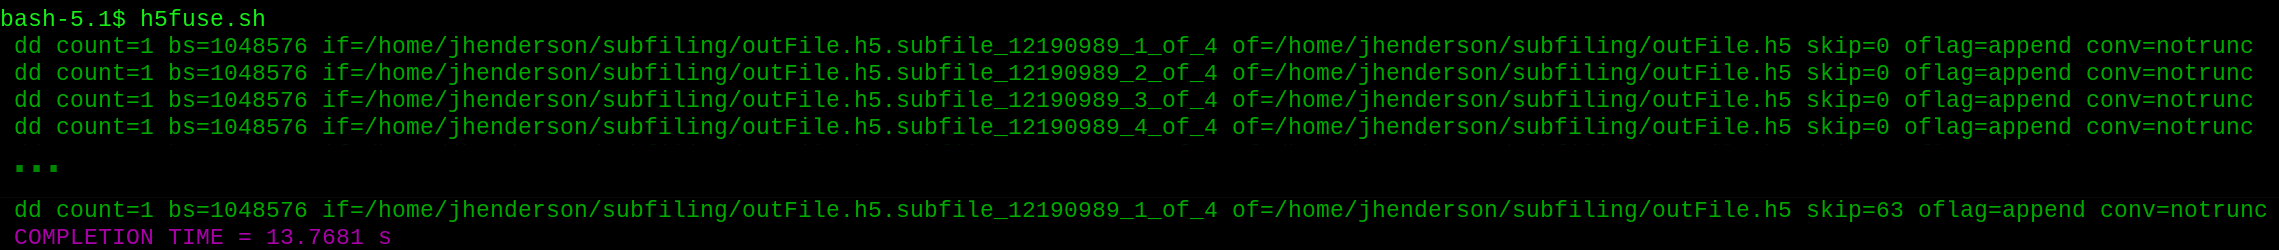
\includegraphics[width=\textwidth]{images/H5fuse_edited.png}}
\caption{Output from H5fuse script}
\label{fig:h5fuse_output}
\end{figure}

\subsection{HDF5 tools support}

There are a few different ways that HDF5's tools can be used with a Subfiling VFD-based
HDF5 file. The most obvious way would be to use the H5fuse tool to convert the Subfiling
VFD-based file into a regular HDF5 file and then utilize HDF5's tools normally.

Alternatively, HDF5's tools can also load and use the Subfiling VFD directly to access one of these files. For example,

\begin{minted}{bash}
# Load the Subfiling VFD by environment variable and
# dump "my_subfiling_file.h5"
HDF5_DRIVER=subfiling h5dump my_subfiling_file.h5
\end{minted}

OR

\begin{minted}{bash}
# Load the Subfiling VFD by FAPL and dump 
# "my_subfiling_file.h5"
h5dump --filedriver=subfiling my_subfiling_file.h5
\end{minted}

The former method should work for most use cases, but the latter approach may be needed
when an HDF5 tool works with more than one file simultaneously and only one of the
files is a Subfiling VFD-based HDF5 file. For example, this method would be needed if
using \texttt{h5repack} to convert a Subfiling file into a different format through
the use of another VFD.

\end{document}